\documentclass{standalone}
\usepackage{xr}
\externaldocument{../Chapter1/Section3/Subsection3/Unet}
\begin{document}
\subsection{Training}

This step is one of the most important since the Convolutional Neural Network (CNN) model coming from the training process will be used for the segmentation of the images.
\\
Before proceeding with the training, the MRI scans and the medical annotation of each patient were manually checked since for some of them there was misregistration between the image and the medical annotation (i.e. the medical annotation did not correspond to the correct slice).
The medical annotations consist of a set of $(x, y)$ points that border the tumor area on the image.
Pixels inside the bordered area were labeled with a value of 255 while the other ones with 0.
\\
The images were then selected and stored in the proper directories, one for the images in DICOM format and one for the ground-truth images stored as 8-bit unsigned integers images.
\\
The training was performed by using a custom data generator which was responsible for providing the right input and ground-truth images, pre-processing them and splitting the images into training and validation sets.
\\
Some data augmentation was also performed on the training set of data, to overcome the lack of data and to reduce overfitting.
It consists in adding slightly modified copies of already existing data, using geometrical transformations such as flipping and rotations of the images.
In this particular case, the images were randomly horizontal or vertical flipped.
\\
In summary, the custom data generator provides the following steps: 
\begin{itemize}
    \item read the input images and ground-truth images from the relative directories
    \item shuffle and split data into training and validation sets
    \item pre-process the input images following the steps described in the previous subsection
    \item normalize and rescale the images
    \item zip the input images with the correct ground-truth images
    \item perform data-augmentation on training set
\end{itemize} 
An example of input and ground-truth images from the training set is shown in Figure \ref{showdataset}.
Instaed, An example of input and ground-truth images from the validation set is shown in Figure \ref{showdataset2}.
In this case no data augmentation is performed.
\\
The network architecture used for this project is a U-Net-like structure made by a contraction and expansion path.
The difference between the original architecture and the one used in this project consists of the use of a so-called \textit{backbone} which refers to the feature extracting network.
Just to clarify this notion, in Figure \ref{fig:unet}, the feature maps (blue boxes) are extracted by a series of Convolutional, ReLu, and Max-pooling layers (denoted by the arrows).
However, one can use various combinations of different layers to extract feature maps. 
So, the combination of layers can create new networks and architectures.
In this case the \textit{backbone} consists of an architecture called \textit{EfficientNetb0}\cite{EfficientNet}.
\\
The loss function is the combination between Dice loss with the binary focal loss.
\\
The algorithm used to minimize the loss function consists of the default \textit{Adam} (Adaptive Moment Estimation) optimizer provided by \textsc{TensorFlow}.
\\
The metric function used to judge the performance during the training of the model was the Dice Similarity Coefficient (DSC).

\begin{figure}[htp]

    \centering
    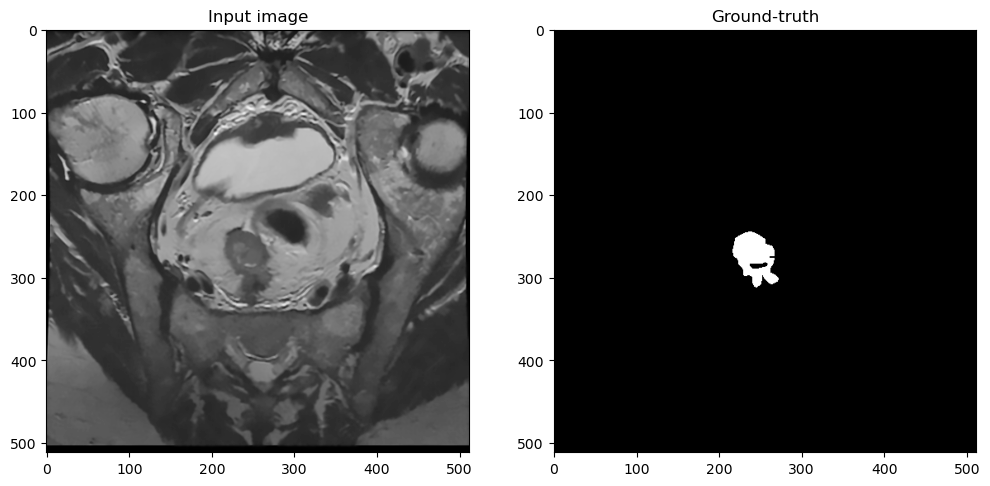
\includegraphics[width=0.9\textwidth]{../images/showdataset.png}
    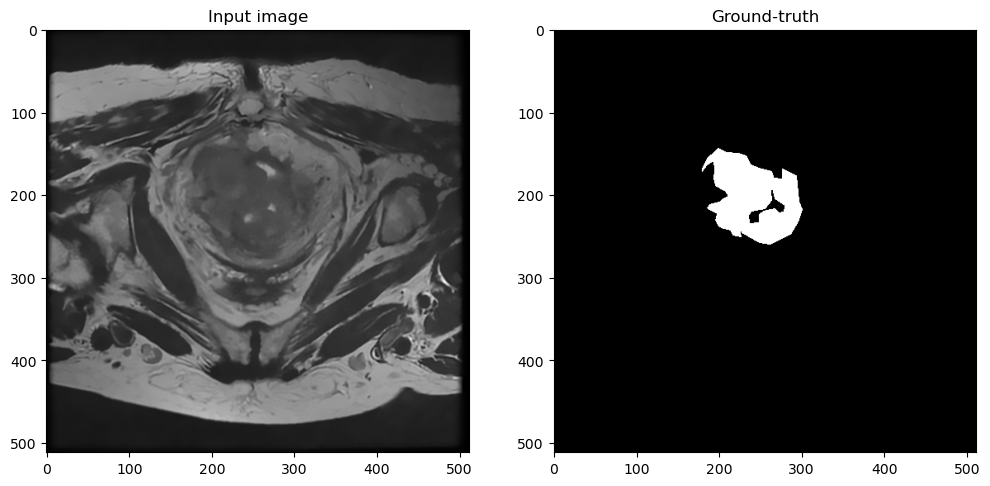
\includegraphics[width=0.9\textwidth]{../images/showdataset1.png}

    \caption{Example of input and ground-truth images from the training set.
    The white area on the ground-truth images represents the tumor area. As you can see, the images are randomly horizontally or vertically flipped. }
    \label{showdataset}
    
    \end{figure}

\begin{figure}[htp]

    \centering
    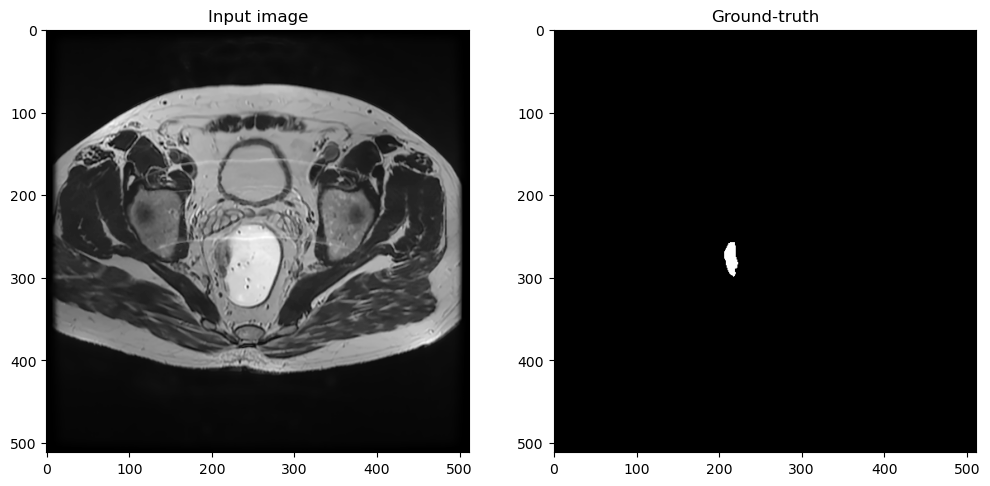
\includegraphics[width=0.9\textwidth]{../images/showdataset2.png}
    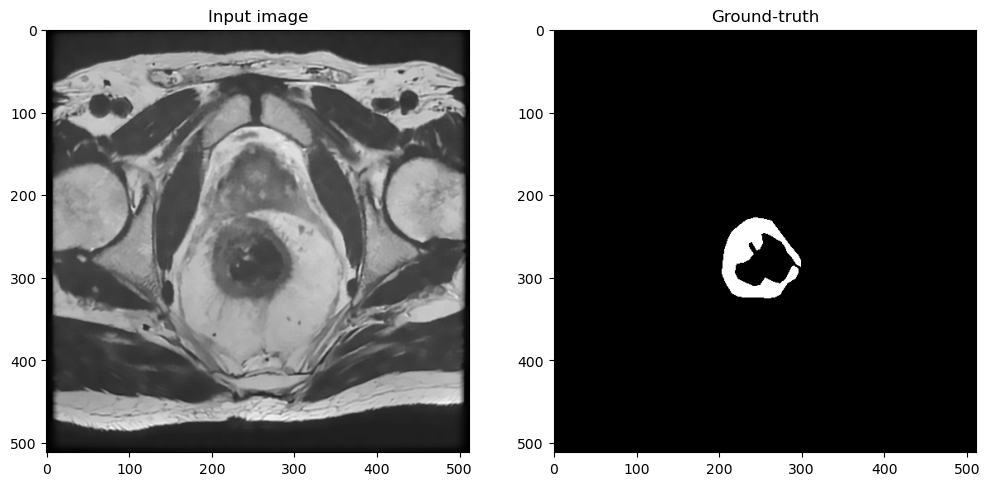
\includegraphics[width=0.9\textwidth]{../images/showdataset3.png}

    \caption{Example of input and ground-truth images from the validation set.The white area on the ground-truth images represents the tumor area. As you can see, no data augmentation was performed on this set}
    \label{showdataset2}
    
    \end{figure}

\end{document}

